\section{Interpolacja Hermite'a}
%\begin{frame}
%{3.8 Interpolacja Hermite'a}

%Więcej o metodzie i jej autorze \\
%(autor: Shayne Waldrom,University of Auckland):\\
%\vspace{5mm}
%https://www.math.auckland.ac.nz/$\sim$waldron/Hermite/he%rmite.html
%\end{frame}

%
\begin{frame}{Interpolacja Hermite'a}
\textcolor{blue}{Dane:}
\begin{itemize}
\item $k+1$ różnych węzłów: $x_{0}, x_{1}, \dots, x_{k}$

\item tzw. krotności węzłów dane liczbami naturalnymi $m_{0}, m_{1},\dots , m_{k}, \displaystyle \sum_{i=0}^{k}m_{i}=n+1$
\end{itemize}
\textcolor{blue}{Szukamy:}

Dla dowolnej funkcji $f$ -- szukamy wielomianu $H_{n}$ stopnia $\leq n,$ \\
takiego, że:

$H_{n}^{(j)}(x_{i})=f^{(j)}(x_{i})$ \quad dla $i=0, 1, \dots , k$ oraz
$j=0, 1, \dots, m_{i}$\\
\vspace{0.5cm}
Krotność mówi nam, ile pochodnych ma być równych.
Gdy $m_{i}=1$ -- interpolacja Lagrange'a.
\end{frame}

\begin{frame}{Rozwiązanie}
Suma krotności $i$ początkowych węzłów interpolacyjnych
\vspace{2mm}
$s(i)=\left\{\begin{array}{l}
0,\ i=0\\
m_{0}+m_{1}+\cdots+m_{i-1},\ i>0
\end{array}\right.$
\vspace{2mm}\\

Zauważmy, że każda liczba 
$0\leq l\leq n$ da się przedstawić w postaci $l=s(i)+j$ gdzie $0 \leq i \leq k$ oraz $0 \leq j \leq m_{i}-1$\\
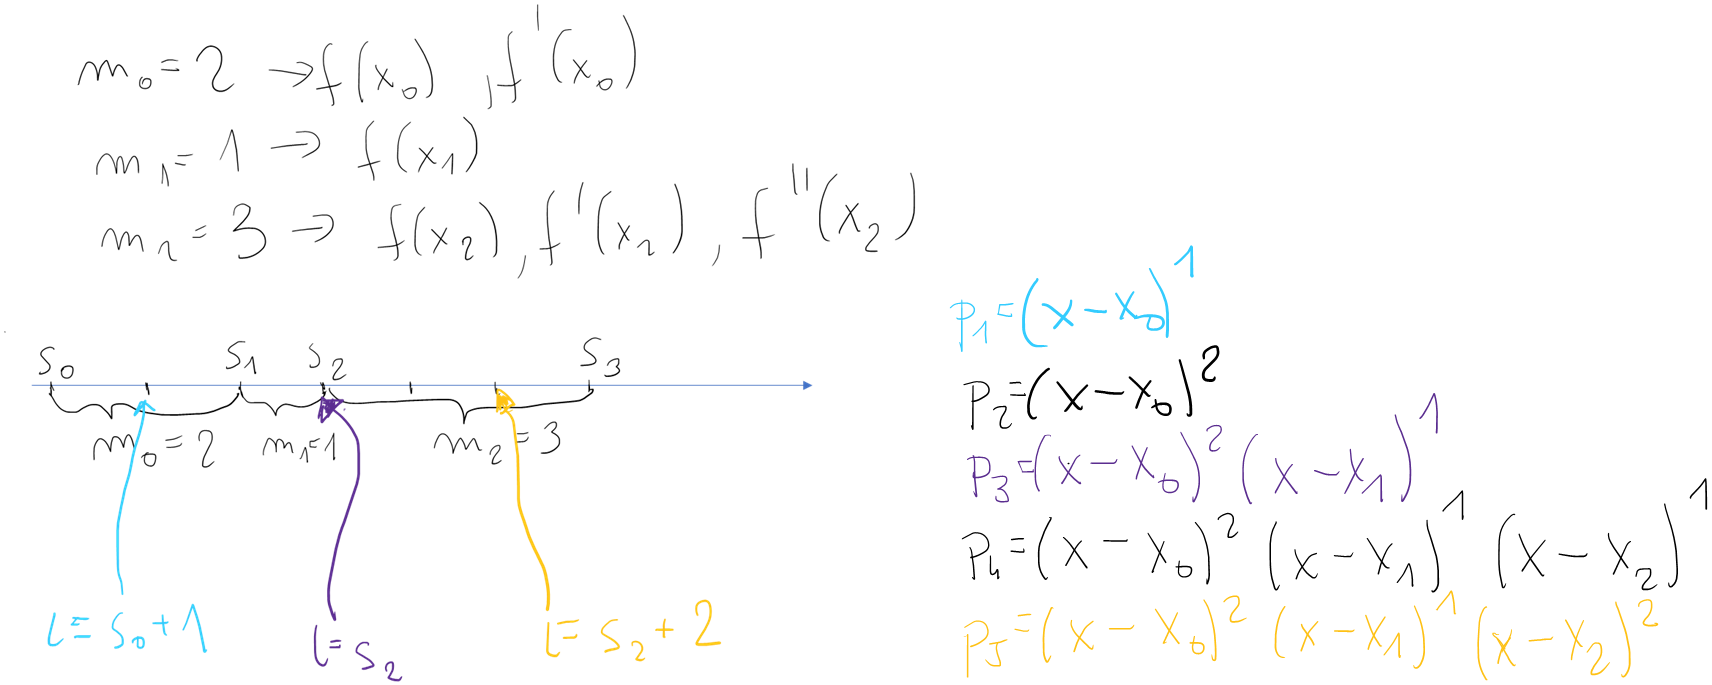
\includegraphics[scale=0.3]{img/3/hermit.png}
\end{frame}
\begin{frame}
\vspace{0.5cm}
Definiujemy wielomiany:\\
$p_{s(0)}(x)=1$

$p_{(s(i)+j)}(x)=(x-x_{0})^{m_{0}}(x-x_{1})^{m_{1}}\ldots(x-x_{i-1})^{m_{i-1}}(x-x_{i})^{j}(\star)$ \\
gdzie: $i=0, 1, \dots, k; \: j=0, 2, \dots , m_{i}-1$ \\
Wtedy szukany wielomian interpolacyjny to kombinacja linowa takich wielomianów (por. postać Newtona)
$$
H_{n}(x)=\sum_{l=0}^{n}b_{l}\cdot p_{l}(x)=\sum_{i=0}^{k}\sum_{j=0}^{m_{i-1}}b_{(s(i)+j)}\cdot p_{(s(i)+j)}(x)
$$
\end{frame}

\begin{frame}
Jak znaleźć współczynniki $b_{l}$:
\begin{itemize}
    \item Tworzymy tablicę ilorazów różnicowych jak w metodzie Newtona.
    \item Tam gdzie nie można utworzyć ilorazu $\rightarrow$ wykorzystujemy informację o pochodnej
\end{itemize}


Przykład dla $m_1=3$
\begin{array}{llllll} 
  x_0 & \color{red} f(x_0) \\ 
  x_1 & f(x_1) & \color{red}  f[x_0,x_1] \\ 
  x_1 & f(x_1) & f'(x_1) & \color{red}  f[x_0,x_1,x_1] \\ 
  x_1 & f(x_1) & f'(x_1) & \frac{f''(x_1)}{2!}& \color{red} f[x_0,x_1,x_1,x_1]\\
  \ldots & \ldots & \ldots & \ldots & \ldots & \ldots\\ 
  x_n & f(x_n) & f[x_{n-1},x_n] & \ldots & \ldots & \color{red}  f[x_0,\ldots,x_n] 
  \end{array}
\end{frame}
%\begin{frame}
%$l$ - ustalone, $l=s(i)+j$
%$$
%H_{n}(x)=\underbrace{A(x)}_{b_{0},{b_{1},\ldots,b}_{l-1}}+b_{l}p_{l}(x)+\underbrace{B(..x)}_{b_{l+1},\ldots,b_{n}}(\star\star)
%$$
%gdzie:
%$A(x)$ - kombinacja liniowa wielomianów $b_i$ o znanych już współczynnikach %$b_{0},{b_{1},\ldots,b}_{l-1}$\\

%\vspace{3mm}
%$B(x)$ - kombinacja liniowa wielomianów $b_i$ o współczynnikach %$b_{l+1},\ldots,b_{n}$
%\end{frame}
%\begin{frame}
%Biorąc pod uwagę (*)
%$$
%p_{l}(x)=p_{(s(i)+j)}(x)=p_{s(i)}(x)(x-x_{i})^{j}
%$$
%oraz dla $m > l$ czyli wielomianów wchodzących w skład $B(x)$, każdy jest %postaci
%$$
%p_{m}(x)=f_m(x)*(x-x_{i})^{k}(***)
%$$
%gdzie $k>j$ oraz $f_m(x)$ zawiera czynniki z(*) dla pozostałych węzłow. \\
%\end{frame}
%\begin{frame}
%różniczkując $(\star\star)$ korzystamy ze wzoru na pochodną iloczynu 

%$$
%(f\cdot g)^{(j)}=f^{(j)}\cdot g+ {n\choose 1} f^{(j-1)}\cdot g^{(1)}+{n\choose %2} f^{(j-2)}\cdot g^{(2)}+f\cdot g^{(j)}
%$$
%oraz faktu, że dla $j\leq k$
%$$
%((x-x_i)^{k})^{(j)}=k\cdot (k-1) ...(k-j+1)(x-x_i)^{k-j}
%$$
%Interesuje nas $H_{n}^{(j)}(x_{i})$\\
%Ze względu na (***) $B^{(j)}(x_i)=0$ i mamy:
%$$
%H_{n}^{(j)}(x_{i})=A^{(j)}(x_{i})+b_{l}p_{s(i)}(x_{i})j!
%$$
%korzystając $\mathrm{z}$:
%$$
%H_{n}^{(j)}(x_{i})=f^{(j)}(x_{i})
%$$
%mamy:
%$$
%b_{l}=\frac{f^{(j)}(x_{i})-A^{(j)}(x_{i})}{p_{s(i)}(x_{i})j!}
%$$

%\end{frame}
